%% LyX 2.0.6 created this file.  For more info, see http://www.lyx.org/.
%% Do not edit unless you really know what you are doing.
\documentclass[slovene]{scrreprt}
\usepackage[T1]{fontenc}
\usepackage[utf8x]{inputenc}
\setcounter{secnumdepth}{3}
\setcounter{tocdepth}{3}
\usepackage{color}
\usepackage{array}
\usepackage{prettyref}
\usepackage{graphicx}
\usepackage{esint}

\makeatletter

%%%%%%%%%%%%%%%%%%%%%%%%%%%%%% LyX specific LaTeX commands.
%% Because html converters don't know tabularnewline
\providecommand{\tabularnewline}{\\}

%%%%%%%%%%%%%%%%%%%%%%%%%%%%%% User specified LaTeX commands.

\usepackage[top=3cm,bottom=3cm,left=3.2cm,right=3.2cm,headsep=10pt,a4paper]{geometry} % Page margins

\usepackage{xcolor,lipsum} % Required for specifying colors by name
\definecolor{ocre}{RGB}{0,56,102} 
\definecolor{lightgray}{RGB}{229,229,229} 
% Font Settings
\usepackage{avant} % Use the Avantgarde font for headings
%\usepackage{times} % Use the Times font for headings
\usepackage{mathptmx} % Use the Adobe Times Roman as the default text font together with math symbols from the Sym­bol, Chancery and Com­puter Modern fonts


\usepackage{microtype} % Slightly tweak font spacing for aesthetics
\usepackage[utf8]{inputenc}
\usepackage[T1]{fontenc} % Use 8-bit encoding that has 256 glyphs
\usepackage[unicode]{hyperref}
\usepackage{empheq}
\usepackage{color}
\usepackage{caption}
\usepackage{afterpage}
\newcommand{\boxeq}[2]{\begin{empheq}[box=\colorbox{ocre!30}]{align}\label{#1}#2\end{empheq}}
\newcommand*{\xdash}[1][8em]{\rule[0.5ex]{#1}{0.55pt}}
\usepackage{makeidx}
\makeindex

% MATHS PACKAGE
\usepackage{amsmath,tikz}
\usetikzlibrary{matrix}
\newcommand*{\horzbar}{\rule[0.05ex]{2.5ex}{0.5pt}}
\usepackage{calc}

% VERBATIM PACKAGE
\usepackage{verbatim}
\usepackage{wrapfig}

%----------------------------------------------------------------------------------------
%	VARIOUS REQUIRED PACKAGES
%----------------------------------------------------------------------------------------

\usepackage{titlesec} % Allows customization of titles

\usepackage{graphicx} % Required for including pictures
\graphicspath{{Pictures/}} % Specifies the directory where pictures are stored

\usepackage{lipsum} % Inserts dummy text

\usepackage{tikz} % Required for drawing custom shapes

\usepackage[slovene]{babel} % English language/hyphenation

\usepackage{enumitem} % Customize lists
\setlist{nolistsep} % Reduce spacing between bullet points and numbered lists

\usepackage{booktabs} % Required for nicer horizontal rules in tables

\usepackage{eso-pic} % Required for specifying an image background in the title page

%\usepackage{draftwatermark}

%----------------------------------------------------------------------------------------
%	MAIN TABLE OF CONTENTS
%----------------------------------------------------------------------------------------

\usepackage{titletoc} % Required for manipulating the table of contents

\contentsmargin{0cm} % Removes the default margin
% Chapter text styling
\titlecontents{chapter}[1.25cm] % Indentation
{\addvspace{15pt}\large\sffamily\bfseries} % Spacing and font options for chapters
{\color{ocre!60}\contentslabel[\Large\thecontentslabel]{1.25cm}\color{ocre}} % Chapter number
{}  
{\color{ocre!60}\normalsize\sffamily\bfseries\;\titlerule*[.5pc]{.}\;\thecontentspage} % Page number
% Section text styling
\titlecontents{section}[1.25cm] % Indentation
{\addvspace{5pt}\sffamily\bfseries} % Spacing and font options for sections
{\contentslabel[\thecontentslabel]{1.25cm}} % Section number
{}
{\sffamily\hfill\color{black}\thecontentspage} % Page number
[]
% Subsection text styling
\titlecontents{subsection}[1.25cm] % Indentation
{\addvspace{1pt}\sffamily\small} % Spacing and font options for subsections
{\contentslabel[\thecontentslabel]{1.25cm}} % Subsection number
{}
{\sffamily\;\titlerule*[.5pc]{.}\;\thecontentspage} % Page number
[] 

%----------------------------------------------------------------------------------------
%	MINI TABLE OF CONTENTS IN CHAPTER HEADS
%----------------------------------------------------------------------------------------

% Section text styling
\titlecontents{lsection}[0em] % Indendating
{\footnotesize\sffamily} % Font settings
{}
{}
{}

% Subsection text styling
\titlecontents{lsubsection}[.5em] % Indentation
{\normalfont\footnotesize\sffamily} % Font settings
{}
{}
{}
 
%----------------------------------------------------------------------------------------
%	PAGE HEADERS
%----------------------------------------------------------------------------------------

\usepackage{fancyhdr} % Required for header and footer configuration

\pagestyle{fancy}
\renewcommand{\chaptermark}[1]{\markboth{\sffamily\normalsize\bfseries\chaptername\ \thechapter.\ #1}{}} % Chapter text font settings
\renewcommand{\sectionmark}[1]{\markright{\sffamily\normalsize\thesection\hspace{5pt}#1}{}} % Section text font settings
\fancyhf{} \fancyhead[LE,RO]{\sffamily\normalsize\thepage} % Font setting for the page number in the header
\fancyhead[LO]{\rightmark} % Print the nearest section name on the left side of odd pages
\fancyhead[RE]{\leftmark} % Print the current chapter name on the right side of even pages
\renewcommand{\headrulewidth}{0.5pt} % Width of the rule under the header
\addtolength{\headheight}{2.5pt} % Increase the spacing around the header slightly
\renewcommand{\footrulewidth}{0pt} % Removes the rule in the footer
\fancypagestyle{plain}{\fancyhead{}\renewcommand{\headrulewidth}{0pt}} % Style for when a plain pagestyle is specified

% Removes the header from odd empty pages at the end of chapters
\makeatletter
\renewcommand{\cleardoublepage}{
\clearpage\ifodd\c@page\else
\hbox{}
\vspace*{\fill}
\thispagestyle{empty}
\newpage
\fi}

%----------------------------------------------------------------------------------------
%	THEOREM STYLES
%----------------------------------------------------------------------------------------

\usepackage{amsmath,amsfonts,amssymb,amsthm} % For math equations, theorems, symbols, etc

\newcommand{\intoo}[2]{\mathopen{]}#1\,;#2\mathclose{[}}
\newcommand{\ud}{\mathop{\mathrm{{}d}}\mathopen{}}
\newcommand{\intff}[2]{\mathopen{[}#1\,;#2\mathclose{]}}
\newtheorem{notation}{Notation}[chapter]

%%%%%%%%%%%%%%%%%%%%%%%%%%%%%%%%%%%%%%%%%%%%%%%%%%%%%%%%%%%%%%%%%%%%%%%%%%%
%%%%%%%%%%%%%%%%%%%% dedicated to boxed/framed environements %%%%%%%%%%%%%%
%%%%%%%%%%%%%%%%%%%%%%%%%%%%%%%%%%%%%%%%%%%%%%%%%%%%%%%%%%%%%%%%%%%%%%%%%%%
\newtheoremstyle{ocrenumbox}% % Theorem style name
{0pt}% Space above
{0pt}% Space below
{\normalfont}% % Body font
{}% Indent amount
{\small\bf\sffamily\color{ocre}}% % Theorem head font
{\;}% Punctuation after theorem head
{0.25em}% Space after theorem head
{\small\sffamily\color{ocre}\thmname{#1}\nobreakspace\thmnumber{\@ifnotempty{#1}{}\@upn{#2}}% Theorem text (e.g. Theorem 2.1)
\thmnote{\nobreakspace\the\thm@notefont\sffamily\bfseries\color{black}---\nobreakspace#3.}} % Optional theorem note
\renewcommand{\qedsymbol}{$\blacksquare$}% Optional qed square

\newtheoremstyle{blacknumex}% Theorem style name
{5pt}% Space above
{5pt}% Space below
{\normalfont}% Body font
{} % Indent amount
{\small\bf\sffamily}% Theorem head font
{\;}% Punctuation after theorem head
{0.25em}% Space after theorem head
{\small\sffamily{\tiny\ensuremath{\blacksquare}}\nobreakspace\thmname{#1}\nobreakspace\thmnumber{\@ifnotempty{#1}{}\@upn{#2}}% Theorem text (e.g. Theorem 2.1)
\thmnote{\nobreakspace\the\thm@notefont\sffamily\bfseries---\nobreakspace#3.}}% Optional theorem note

\newtheoremstyle{blacknumbox} % Theorem style name
{0pt}% Space above
{0pt}% Space below
{\normalfont}% Body font
{}% Indent amount
{\small\bf\sffamily}% Theorem head font
{\;}% Punctuation after theorem head
{0.25em}% Space after theorem head
{\small\sffamily\thmname{#1}\nobreakspace\thmnumber{\@ifnotempty{#1}{}\@upn{#2}}% Theorem text (e.g. Theorem 2.1)
\thmnote{\nobreakspace\the\thm@notefont\sffamily\bfseries---\nobreakspace#3.}}% Optional theorem note

%%%%%%%%%%%%%%%%%%%%%%%%%%%%%%%%%%%%%%%%%%%%%%%%%%%%%%%%%%%%%%%%%%%%%%%%%%%
%%%%%%%%%%%%% dedicated to non-boxed/non-framed environements %%%%%%%%%%%%%
%%%%%%%%%%%%%%%%%%%%%%%%%%%%%%%%%%%%%%%%%%%%%%%%%%%%%%%%%%%%%%%%%%%%%%%%%%%
\newtheoremstyle{ocrenum}% % Theorem style name
{5pt}% Space above
{5pt}% Space below
{\normalfont}% % Body font
{}% Indent amount
{\small\bf\sffamily\color{ocre}}% % Theorem head font
{\;}% Punctuation after theorem head
{0.25em}% Space after theorem head
{\small\sffamily\color{ocre}\thmname{#1}\nobreakspace\thmnumber{\@ifnotempty{#1}{}\@upn{#2}}% Theorem text (e.g. Theorem 2.1)
\thmnote{\nobreakspace\the\thm@notefont\sffamily\bfseries\color{black}---\nobreakspace#3.}} % Optional theorem note
\renewcommand{\qedsymbol}{$\blacksquare$}% Optional qed square
\makeatother

% Defines the theorem text style for each type of theorem to one of the three styles above
\newcounter{dummy} 
\numberwithin{dummy}{section}
\theoremstyle{ocrenumbox}
\newtheorem{theoremeT}[dummy]{Theorem}
\newtheorem{problem}{Problem}[chapter]
\newtheorem{exerciseT}{Exercise}[chapter]
\theoremstyle{blacknumex}
\newtheorem{exampleT}{Example}[chapter]
\theoremstyle{blacknumbox}
\newtheorem{vocabulary}{Vocabulary}[chapter]
\newtheorem{definitionT}{Naloga}[section]
\newtheorem{corollaryT}[dummy]{Corollary}
\theoremstyle{ocrenum}
\newtheorem{proposition}[dummy]{Računski zgled}

%----------------------------------------------------------------------------------------
%	DEFINITION OF COLORED BOXES
%----------------------------------------------------------------------------------------

\RequirePackage[framemethod=default]{mdframed} % Required for creating the theorem, definition, exercise and corollary boxes

% Theorem box
\newmdenv[skipabove=7pt,
skipbelow=7pt,
backgroundcolor=black!5,
linecolor=ocre,
innerleftmargin=5pt,
innerrightmargin=5pt,
innertopmargin=5pt,
leftmargin=0cm,
rightmargin=0cm,
innerbottommargin=5pt]{tBox}

% Exercise box	  
\newmdenv[skipabove=7pt,
skipbelow=7pt,
rightline=false,
leftline=true,
topline=false,
bottomline=false,
backgroundcolor=ocre!10,
linecolor=ocre,
innerleftmargin=5pt,
innerrightmargin=5pt,
innertopmargin=5pt,
innerbottommargin=15pt,
leftmargin=0cm,
rightmargin=0cm,
linewidth=4pt]{eBox}	

% Definition box
\newmdenv[
skipabove=7pt,
skipbelow=7pt,
rightline=false,
leftline=false,
topline=true,
bottomline=true,
linecolor=ocre,
innerleftmargin=0pt,
innerrightmargin=0pt,
innertopmargin=15pt,
leftmargin=0cm,
rightmargin=0cm,
linewidth=1pt,
innerbottommargin=7pt]{dBox}	

% Corollary box
\newmdenv[skipabove=7pt,
skipbelow=7pt,
rightline=false,
leftline=true,
topline=true,
bottomline=true,
linecolor=red,
backgroundcolor=black!5,
innerleftmargin=5pt,
innerrightmargin=5pt,
innertopmargin=5pt,
leftmargin=0cm,
rightmargin=0cm,
linewidth=4pt,
innerbottommargin=5pt]{cBox}

% Creates an environment for each type of theorem and assigns it a theorem text style from the "Theorem Styles" section above and a colored box from above
\newenvironment{theorem}{\begin{tBox}\begin{theoremeT}}{\end{theoremeT}\end{tBox}}
\newenvironment{exercise}{\begin{eBox}\begin{exerciseT}}{\hfill{\color{ocre}\tiny\ensuremath{\blacksquare}}\end{exerciseT}\end{eBox}}				  
\newenvironment{definition}{\begin{dBox}\begin{definitionT}}{\end{definitionT}\end{dBox}}	
\newenvironment{example}{\begin{exampleT}}{\hfill{\tiny\ensuremath{\blacksquare}}\end{exampleT}}		
\newenvironment{corollary}{\begin{cBox}\begin{corollaryT}}{\end{corollaryT}\end{cBox}}	

%----------------------------------------------------------------------------------------
%	REMARK ENVIRONMENT
%----------------------------------------------------------------------------------------

\newenvironment{remark}{\par\vspace{10pt}\small % Vertical white space above the remark and smaller font size
\begin{list}{}{
\leftmargin=25pt % Indentation on the left
\rightmargin=0pt}\item\ignorespaces % Indentation on the right
\makebox[-2.5pt]{\begin{tikzpicture}[overlay]
\node[draw=ocre!60,line width=1pt,circle,fill=ocre!25,font=\sffamily\bfseries,inner sep=2pt,outer sep=0pt] at (-15pt,0pt){\textcolor{ocre}{$\bigstar$}};\end{tikzpicture}} % Orange R in a circle
\advance\baselineskip -1pt}{\end{list}\vskip5pt} % Tighter line spacing and white space after remark

%----------------------------------------------------------------------------------------
%	SECTION NUMBERING IN THE MARGIN
%----------------------------------------------------------------------------------------

\makeatletter
\renewcommand{\@seccntformat}[1]{\llap{\textcolor{ocre}{\csname the#1\endcsname}\hspace{1em}}}                    
\renewcommand{\section}{\@startsection{section}{1}{\z@}
{-4ex \@plus -1ex \@minus -.4ex}
{1ex \@plus.2ex }
{\normalfont\large\sffamily\bfseries}}
\renewcommand{\subsection}{\@startsection {subsection}{2}{\z@}
{-3ex \@plus -0.1ex \@minus -.4ex}
{0.5ex \@plus.2ex }
{\normalfont\sffamily\bfseries}}
\renewcommand{\subsubsection}{\@startsection {subsubsection}{3}{\z@}
{-2ex \@plus -0.1ex \@minus -.2ex}
{.2ex \@plus.2ex }
{\normalfont\small\sffamily\bfseries}}                        
\renewcommand\paragraph{\@startsection{paragraph}{4}{\z@}
{-2ex \@plus-.2ex \@minus .2ex}
{.1ex}
{\normalfont\small\sffamily\bfseries}}

%----------------------------------------------------------------------------------------
%	HYPERLINKS IN THE DOCUMENTS
%----------------------------------------------------------------------------------------

% For an unclear reason, the package should be loaded now and not later
\usepackage{hyperref}
\hypersetup{hidelinks,backref=true,pagebackref=true,hyperindex=true,colorlinks=true,breaklinks=true,urlcolor= ocre,linkcolor=ocre,bookmarks=true,bookmarksopen=false,pdftitle={Title},pdfauthor={Author}}

%----------------------------------------------------------------------------------------
%	CHAPTER HEADINGS
%----------------------------------------------------------------------------------------

% The set-up below should be (sadly) manually adapted to the overall margin page septup controlled by the geometry package loaded in the main.tex document. It is possible to implement below the dimensions used in the goemetry package (top,bottom,left,right)... TO BE DONE

\newcommand{\thechapterimage}{}
\newcommand{\chapterimage}[1]{\renewcommand{\thechapterimage}{#1}}

% Numbered chapters with mini tableofcontents
\def\thechapter{\arabic{chapter}}
\def\@makechapterhead#1{
\thispagestyle{empty}
{\centering \normalfont\sffamily
\ifnum \c@secnumdepth >\m@ne
\if@mainmatter
\startcontents
\begin{tikzpicture}[remember picture,overlay]
\node at (current page.north west)
{\begin{tikzpicture}[remember picture,overlay]
\node[anchor=north west,inner sep=0pt] at (0,0) {\includegraphics[width=\paperwidth]{\thechapterimage}};
%%%%%%%%%%%%%%%%%%%%%%%%%%%%%%%%%%%%%%%%%%%%%%%%%%%%%%%%%%%%%%%%%%%%%%%%%%%%%%%%%%%%%
% Commenting the 3 lines below removes the small contents box in the chapter heading
%\fill[color=ocre!10!white,opacity=.6] (1cm,0) rectangle (8cm,-7cm);
%\node[anchor=north west] at (1.1cm,.35cm) {\parbox[t][8cm][t]{6.5cm}{\huge\bfseries\flushleft \printcontents{l}{1}{\setcounter{tocdepth}{2}}}};
\draw[anchor=west] (3cm,-4cm) node [rounded corners=20pt,fill=ocre!10!white,text opacity=1,draw=ocre,draw opacity=1,line width=1.5pt,fill opacity=.6,inner sep=12pt]{\huge\sffamily\bfseries\textcolor{black}{\thechapter. #1\strut\makebox[22cm]{}}};
%%%%%%%%%%%%%%%%%%%%%%%%%%%%%%%%%%%%%%%%%%%%%%%%%%%%%%%%%%%%%%%%%%%%%%%%%%%%%%%%%%%%%
\end{tikzpicture}};
\end{tikzpicture}}
\par\vspace*{100\p@}
\fi
\fi}

% Unnumbered chapters without mini tableofcontents (could be added though) 
\def\@makeschapterhead#1{
\thispagestyle{empty}
{\centering \normalfont\sffamily
\ifnum \c@secnumdepth >\m@ne
\if@mainmatter
\begin{tikzpicture}[remember picture,overlay]
\node at (current page.north west)
{\begin{tikzpicture}[remember picture,overlay]
\node[anchor=north west,inner sep=0pt] at (0,0) {\includegraphics[width=\paperwidth]{\thechapterimage}};
\draw[anchor=west] (3cm,-4cm) node [rounded corners=20pt,fill=ocre!10!white,fill opacity=.6,inner sep=12pt,text opacity=1,draw=ocre,draw opacity=1,line width=1.5pt]{\huge\sffamily\bfseries\textcolor{black}{#1\strut\makebox[22cm]{}}};
\end{tikzpicture}};
\end{tikzpicture}}
\par\vspace*{80\p@}
\fi

\fi
}
\makeatother
 % Insert the commands.tex file which contains the majority of the structure behind the template

\newcommand{\beq}{\begin{equation}}
\newcommand{\eeq}{\end{equation}}   
\renewcommand{\arraystretch}{1.5}

\newcommand{\usk}{\mbox()}
\newcommand{\micro}{\mu}
\newcommand{\metre}{\mathrm{m}}
\newcommand{\kilo}{\mathrm{k}}
\newcommand{\hertz}{\mathrm{Hz}}
\newcommand{\milli}{\mathrm{m}}
\newcommand{\centi}{\mathrm{c}}
\usepackage{subfig}
\usepackage{parskip}


%Copy-paste iz stare skripte.. 


\usepackage[tikz]{bclogo}
\usepackage{graphicx}
\usepackage{xcolor}
\definecolor{darkblue}{rgb}{0,0,0.5} 
\usepackage{transparent}
\usepackage{import}

%\usepackage[thinspace,amssymb]{SIunits}




%\renewcommand{\capfont}{\normalfont\small} 

%\newcommand{\stevedeli}[1]{\phantom{.}{\small\begin{bclogo}[noborder = true,couleur=gray!10,logo=\bclambe]{Ste vedeli?}{#1}\end{bclogo}}\phantom{.}}
%\newcommand{\zanimivo}[2]{\phantom{.}{\small\begin{bclogo}[noborder = true,couleur=gray!10,logo=\bclampe]{#1}{#2}\end{bclogo}}\phantom{.}}
%\newcommand{\literatura}[1]{\phantom{.}\begin{bclogo}[couleur=gray!10,arrondi=0.1,logo=\bcbook]{Literatura}{#1}\end{bclogo}\phantom{.}}

%\newcounter{exercise}[chapter]
%\renewcommand{\theexercise}{\thechapter .\arabic{exercise}}

%\newcommand{\naloga}[2]{\refstepcounter{exercise}
%\label{#1}
%\phantom{.}{\small\begin{bclogo}[couleur=blue!30,arrondi=0.1,logo=\bccrayon,ombre=True,couleurOmbre=black!60,barre=snake]{Naloga  \theexercise}{#2}\end{bclogo}}\vspace{1mm}}


%\graphicspath{{/Users/andrej/Documents/Fotonika/skripta/slike/}}
\graphicspath{{./slike/}}

%\usepackage{prettyref}
%\newrefformat{tab}{Tabela\,\ref{#1}}
%\newrefformat{fig}{Slika\,\ref{#1}}
%\newrefformat{eq}{En.\,\textup{\ref{#1}}}

%\usepackage[uline]{hhtensor}


%\newcommand{\matT}[1] {\matr{\boldsymbol{#1}}^{T}}
%\newcommand{\matI}[1] {\matr{\boldsymbol{#1}}^{-1}}
%\newcommand{\mat}[1] {\matr{\boldsymbol{#1}}}
%\newcommand{\ve}[1] {\boldsymbol{#1}}
%\newcommand{\uve}[1] {\widehat{\boldsymbol{#1}}}
%\newcommand{\dd} {\mathrm{d}}
%\newcommand{\Tr}{\textrm{Tr}}

%\newcommand{\tagarray}{%
%\mbox{}\refstepcounter{equation}%
%$(\theequation)$%
%}

%\renewcommand\Re{\operatorname{Re}}
%\renewcommand\Im{\operatorname{Im}}


\@ifundefined{showcaptionsetup}{}{%
 \PassOptionsToPackage{caption=false}{subfig}}
\usepackage{subfig}
\makeatother

\usepackage{babel}
\begin{document}

\chapter{Koherentni snopi svetlobe}

Pri obravnavi elektromagnetnega valovanja zelo pogosto uporabljamo
približek ravnih valov. Ti so v smeri pravokotno na smer širjenja
neomejeni in so lahko le idealizacija. Čim raven val omejimo z odprtino
v zaslonu, dobimo snop svetlobe. V snopu svetlobe valovna čela niso
ravna in snop ni vzporeden, ampak se zaradi uklona širi (slika \ref{fig:Uklon-na-re=00017Ei}).
\begin{figure}
\centering\small
\input{slike/lom_na_rezi.pdf_tex}

\caption{\label{fig:Uklon-na-re=00017Ei}Omejen snop dobimo z uklonom ravnega
vala na odprtini. Osenčeno območje prestavlja geometrijsko sliko sence.
Kot širjenja valovanja v daljnem polju ($z\gg b=a^{2}/\lambda$) je
obratno sorazmeren s širino odprtine $\theta\simeq\frac{\lambda}{a}$.
\textcolor{red}{Ali je slika v redu? Namerno taka? Jaz bi uklonila
tudi fronte.}}
\end{figure}
\\


V veliki oddaljenosti od zaslona lahko za izračun polja uporabimo
Fraunhoferjevo uklonsko teorijo. Vendar za hitro oceno kota širjenja
snopa podrobnega računa niti ne potrebujemo. Velja približno 
\begin{equation}
\theta\simeq\frac{\lambda}{a},
\end{equation}
kjer je $a$ polmer odprtine v zaslonu. Opis polja v bližini zaslona
je zahtevnejši, treba je uporabiti Fresnelov približek. Iz slike \ref{fig:Uklon-na-re=00017Ei}
lahko ocenimo, da seže območje bližnjega polja do razdalje 
\begin{equation}
b\simeq\frac{a}{\theta}=\frac{a^{2}}{\lambda}.
\end{equation}


Včasih taki približni oceni zadoščata. Bolj kvantitativen opis omejenih
snopov bi lahko dobili s Fraunhoferjevo in Fresnelevo uklonsko teorijo,
kar pa ni najudobnejša pot. Lotimo se naloge raje preko približka
obosne valovne enačbe.


\section{Obosna valovna enačba}

Pričnimo s časovno neodvisno valovno enačbo za monokromatsko valovanje
s frekvenco $\omega$ (Helmholtzova enačba, \ref{eq:Helmholtz}):
\begin{equation}
\nabla^{2}E+k^{2}E=0,\label{eq:valovna-ena=00010Dba}
\end{equation}
kjer je $k=n\omega/c_{0}$ valovno število in $n$ lomni količnik
sredstva, po katerem se valovanje širi. Zaradi enostavnosti obravnavajmo
le eno polarizacijo, tako da je$E$ kar skalar. Iščemo rešitev za
omejen snop, ki se širi približno vzdolž osi $z$. Zapišimo jo v obliki
\begin{equation}
E=E_{0}\psi(\ve{r},z)e^{ikz},\label{eq:ravni-val-nastavek}
\end{equation}
kjer je $\ve{r}$ krajevni vektor v ravnini $xy$. Glavni del odvisnosti
od koordinate $z$ smo zapisali v faktorju $e^{ikz}$, tako da lahko
privzamemo, da se $\psi$ v smeri $z$ le počasi spreminja. Vstavimo
gornji nastavek v Helmoltzovo enačbo (\prettyref{eq:valovna-ena=00010Dba})
in pri tem zanemarimo druge odvode po $z$, saj je $\partial^{2}\psi/\partial z^{2}$
majhen v primerjavi s $k\partial\psi/\partial z$ in $k^{2}\psi$.
Zaenkrat obravnavajmo le radialno simetrične rešitve. Dobimo obosno
ali paraksialno valovno enačbo

\begin{equation}
\nabla_{\perp}^{2}\psi=-2ik{\frac{{\partial\psi}}{{\partial z}}}.\label{eq:obosna-valovna-ena=00010Dba}
\end{equation}
Opazimo, da je obosna valovna enačba enaka Schr\"{o}dingerjevi enačba
za prost delec v dveh dimenzijah, v kateri ima koordinata $z$ vlogo
časa. Omejenemu snopu v kvantni mehaniki ustreza lokaliziran delec
- valovni paket. Ta se s časom širi, kar v optiki ustreza pojavu uklona.\\


Ena družina rešitev, ki v kvantni mehaniki predstavlja lastne funkcije
energije in gibalne količine, so spet ravni valovi 
\begin{equation}
\psi=e^{ik_{1}x+ik_{2}y}\, e^{-i\beta z}.\label{eq:ravni-val-nastavek-obosni}
\end{equation}
Pri tem $\beta$ ustreza energiji v kvantni mehaniki, $k_{1}$ in
$k_{2}$ pa komponentama gibalne količine. Da bo gornji nastavek rešitev
obosne valovne enačbe \ref{eq:obosna-valovna-ena=00010Dba}, mora
veljati 
\begin{equation}
\beta=\frac{k_{1}^{2}+k_{2}^{2}}{2k}.
\end{equation}
Ko vstavimo nastavek za $\psi$ v izraz za celotno polje $E$ (\prettyref{eq:ravni-val-nastavek}),
dobimo raven val, za katerega velja 
\begin{equation}
k_{3}=k-\beta=k-\frac{k_{1}^{2}+k_{2}^{2}}{2k},\label{eq:k3-razvoj}
\end{equation}
 pri čemer je $k_{3}$ vzdolžna komponenta valovnega vektorja, $k_{1}$in
$k_{2}$ prečni komponenti, $k$ pa valovno število. \\


Za ravni val, ki je rešitev prvotne točne valovne enačbe \ref{eq:valovna-ena=00010Dba}
(in ne obosnega približka), velja 
\begin{equation}
k_{3}=\sqrt{k^{2}-(k_{1}^{2}+k_{2}^{2})}.\label{eq:k3-to=00010Dno}
\end{equation}
Očitno dobimo enačbo \prettyref{eq:k3-razvoj} iz enačbe \prettyref{eq:k3-to=00010Dno}
z razvojem korena za majhne vrednosti prečnih komponent valovnega
vektorja, kar seveda ni nič nepričakovanega. Ta ugotovitev nam tudi
pove, da je približek obosne enačbe dober, kadar je razmerje prečne
in vzdolžne komponente valovnega vektorja majhno. Takrat je majhen
tudi kot širjenja snopa in v razvoju lahko zanemarimo člene, višje
od kvadratnih. To pa je tudi območje veljavnosti Fresneleve uklonske
teorije, zato rešitve obosne valovne dajo enako dober približek.

\zanimivo{Fouriereva optika}{Časovno odvisnost poljubnega začetnega
stanja v kvantni mehaniki navadno izračunamo tako, da v nekem začetnem
trenutku paket razvijemo po lastnih stanjih energije - ravnih valovih.
Rešitev v poljubnem kasnejšem trenutku je potem dana v obliki Fourierevega
integrala. Ta pot je zelo uporabna tudi v optiki in je osnova sklopa
računskih metod, znanih pod imenom Fouriereva optika. V našem primeru
z njo brez težav pridemo nazaj do Fresneleve uklonske formule.}


\section{Osnovni Gaussov snop}

Naša naloga je poiskati rešitve obosne enačbe, ki popišejo omejene
snope. Iz kvantne mehanike vemo, da je najbolj lokaliziran in se najpočasneje
širi valovni paket Gaussove oblike. Zato poskusimo najti rešitev obosne
enačbe \ref{eq:obosna-valovna-ena=00010Dba} v obliki 
\begin{equation}
\psi(r,z)=e^{-\frac{kr^{2}}{2}\alpha(z)}\, e^{-i\phi(z)},\label{eq:gaussov-snop-nastavek}
\end{equation}
kjer funkcija $\alpha(z)$ meri, kako se snop širi v prečni smeri,
$\phi(z)$ pa opisuje počasno spreminjanje faze snopa vzdolž osi $z$.
Vstavimo nastavek \ref{eq:gaussov-snop-nastavek} v enačbo \ref{eq:obosna-valovna-ena=00010Dba}.
Velja 
\begin{equation}
\nabla_{\perp}^{2}\psi=\frac{1}{r}\frac{\partial}{\partial r}\, r\,\frac{\partial\psi}{\partial r}=k\alpha(k\alpha r^{2}-2)\psi
\end{equation}
 in 
\begin{equation}
\frac{\partial\psi}{\partial z}=(-\frac{kr^{2}}{2}\alpha^{\prime}-i\phi^{\prime})\psi.
\end{equation}
 Tako iz obosne enačbe \ref{eq:obosna-valovna-ena=00010Dba} dobimo
\begin{equation}
k\alpha(k\alpha r^{2}-2)=ik(k\alpha^{\prime}r^{2}+2i\phi^{\prime}).
\end{equation}
 Gornji izraz mora veljati pri vsakem $r$, zato morajo biti koeficienti
pri $r^{2}$ in konstanti posebej enaki 0: 
\begin{equation}
\alpha^{2}-i\alpha^{\prime}=0\mbox{\hskip1cm in \hskip1cm}\phi^{\prime}=\alpha
\end{equation}
 Z integracijo dobimo najprej 
\begin{equation}
\frac{1}{\alpha}=z_{0}+iz,\label{eq:alpha}
\end{equation}
kjer je $z_{0}$ integracijska konstanta, ki jo s primerno izbiro
izhodišča lahko naredimo realno. Integriramo še enačbo za fazo 
\begin{equation}
\phi=\int_{0}^{z}\,\frac{dz}{z_{0}+iz}=-i\ln(1+i\frac{z}{z_{0}}).
\end{equation}
 Predpisali smo, da je faza v izhodišču (pri $z=0$) enaka 0. Tako
imamo 
\begin{eqnarray}
\psi & = & \exp\left[-\frac{kr^{2}}{2(z_{0}+iz)}\right]\,\exp\left[-\ln(1+i\frac{z}{z_{0}})\right]\nonumber \\
 & = & \frac{1}{1+i\frac{z}{z_{0}}}\,\exp\left[-\frac{kr^{2}z_{0}}{2(z_{0}^{2}+z^{2})}+\frac{ikr^{2}z}{2(z_{0}^{2}+z^{2})}\right].\label{eq:gaussov-snop-vmesni}
\end{eqnarray}
 Realni del eksponenta opisuje širjenje snopa. Vpeljimo polmer snopa
$w$: 
\begin{equation}
w^{2}=\frac{2z_{0}}{k}\left[1+(\frac{z}{z_{0}})^{2}\right]=w_{0}^{2}\left[1+(\frac{z}{z_{0}})^{2}\right],\label{eq:w}
\end{equation}
kjer je $w_{0}$ polmer snopa na najožjem delu, to je v izhodišču.
Najožji del imenujem\textcolor{black}{o grlo snopa}. Odvisnost $w$
od $z$ je hiperbolična, pri čemer je $z_{0}$ polovična dolžina grla
oziroma razdalja, pri kateri preide snop v asimptotično enakomerno
širjenje. Pri $z_{0}$ tudi preidemo v območje veljavnosti Fraunhoferjevega
uklonskega približka. Med $w_{0}$ in $z_{0}$ velja zveza 
\begin{equation}
z_{0}=\frac{\pi w_{0}^{2}}{\lambda}.\label{eq:z0}
\end{equation}


Iz izraza \ref{eq:w} za $w$ razberemo še kot divergence snopa v
asimptotičnem območju: 
\begin{equation}
\theta=2\frac{w_{0}}{z_{0}}=\frac{2\lambda}{\pi w_{0}}.\label{eq:divergenca-snopa}
\end{equation}
 Dobljeni izrazi so v skladu z ocenami, ki smo jih napravili v začetku
poglavja, pri čemer je faktor $2/\pi$ pri divergenci značilen za
Gaussov snop, ki ima od vseh možnih oblik najmanjšo divergenco.

Vrnimo se k imaginarnemu delu eksponenta v drugi enačbi \ref{eq:gaussov-snop-vmesni}.
Količina 
\begin{equation}
R=z[1+(\frac{z_{0}}{z})^{2}]\label{eq:R}
\end{equation}
 meri ukrivljenost valovnih front snopa v razdalji $z$. To najlažje
uvidimo, če krogelni val razvijemo po majhnih odmikih $r$ od osi
$z$: 
\begin{equation}
\frac{1}{R}e^{ikR}=\frac{1}{R}e^{ik\sqrt{z^{2}+r^{2}}}\simeq\frac{1}{R}e^{ik(z+\frac{r^{2}}{2R})}.\label{eq:krogelni-val}
\end{equation}
 Upoštevali smo, da je na osi $z=R$.

Faktor pred eksponentom v izrazu \ref{eq:gaussov-snop-vmesni} meri
zmanjševanje amplitude snopa in s tem poskrbi za ohranitev energijskega
toka, poleg tega pa da še dodatno spremembo faze. Zapišimo ga v obliki
\begin{equation}
\frac{1}{1+i\frac{z}{z_{0}}}=\frac{1}{\sqrt{1+(\frac{z_{0}}{z})^{2}}}e^{-i\eta(z)}=\frac{w_{0}}{w}e^{-i\eta(z)},
\end{equation}
 
\begin{equation}
\eta(z)=\arctan(\frac{z}{z_{0}}).\label{eq:eta}
\end{equation}
 Dodatna faza $\eta$ je posledica povečane fazne hitrosti valovanja,
kadar je omejeno v prečni smeri. Pojav je najizrazitejši v bližini
grla snopa. Srečamo ga tudi pri valovanju po valovodih.
\begin{figure}
\centering\small
\def\svgwidth{0.6\textwidth}
\input{slike/ravni_val.pdf_tex}
\def\svgwidth{0.6\textwidth}
\input{slike/gaussov_snop.pdf_tex}
\def\svgwidth{0.6\textwidth}
\input{slike/krogelni_val.pdf_tex}


\caption{\label{fig:ravni-Gaussov-krogelni-val}Ravni val, Gaussov snop ter
krogelni val. Pri majhnih razdaljah od grla je Gaussov snop podoben
ravnemu valu, pri velikih razdaljah pa krogelnemu valu. Divergenca
snopa je $w_{0}/z_{0}$.}


\end{figure}


S tem lahko končno zapišemo izraz za polje \textit{osnovnega Gaussovega
snopa}: 
\begin{equation}
E=E_{0}\,\frac{w_{0}}{w}\exp\{i[kz-\eta(z)]-r^{2}[\frac{1}{w^{2}(z)}-\frac{ik}{2R(z)}]\}.\label{eq:gaussov-snop}
\end{equation}
Na sliki \ref{fig:ravni-Gaussov-krogelni-val} so shematsko prikazani
ravni val, Gaussov snop (\prettyref{eq:gaussov-snop}) in krogelni
val (\prettyref{eq:krogelni-val}). Vidimo, da je za majhne $z$ Gaussov
snop podoben ravnemu valu, medtem ko je za velike $z$ podoben krogelnemu
valu, pri tem pa je faza Gaussovega snopa pri $z\gg z_{0}$ zamaknjena
za $\pi/2$ glede na ravni in krogelni val. 

\naloga{naloga-širina-snopa}{Pokaži, da je znotraj širine snopa
$w$ približno $87\%$ svetlobnega toka. Namig: upoštevaj, da je delež
svetlobnega toka sorazmeren z $\propto\int_{0}^{w}\exp(-2r^{2}/w^{2})r\, dr$.}

Za računanje je prikladno vpeljati še \textit{kompleksni krivinski
radij} $q$: 
\begin{equation}
\frac{1}{q(z)}=\frac{1}{R}+i\frac{2}{kw^{2}}=i\alpha(z).\label{eq:q-inv}
\end{equation}
 Ker je po \ref{eq:alpha} funkcija $1/\alpha(z)$ linearna, je taka
tudi odvisnost kompleksnega krivinskega radija od $z$: 
\begin{equation}
q(z)=z-iz_{0}.\label{eq:q}
\end{equation}


\naloga{naloga-širina-snopa}{Pokaži, da je največja ukrivljenost
snopa (namanjši $R$) ravno pri $z=\pm z_{0}$.}


\section{Snopi višjega reda}

Osnovni Gaussov snop je le ena od mnogih v prečni smeri omejenih rešitev
obosne valovne enačbe. V kartezičnih koordinatah jo rešijo tudi funkcije
\begin{equation}
\psi_{n,m}(x,y)=\frac{w_{0}}{w}H_{n}(\frac{\sqrt{2}x}{w})H_{m}(\frac{\sqrt{2}y}{w})\exp[\frac{ik(x^{2}+y^{2})}{2q}-i\eta_{n,m}],\label{eq:Gauss-Hermitevi}
\end{equation}
kjer so $H_{n}$ Hermitevi polinomi stopnje $n$. V to se brez težav
prepričamo, če izraz vstavimo v obosno enačbo in upoštevamo, da Hermitevi
polinomi zadoščajo enačbi 
\begin{equation}
H_{n}^{\prime\prime}-2H_{n}^{\prime}+2nH_{n}=0.
\end{equation}
Osnovni Gaussov snop je očitno poseben primer gornje rešitve za $m=n=0$.
Polmer snopa $w(z)$ in kompleksni krivinski radij $q(z)$ sta za
vse $m$ in $n$ enaka kot za osnovni snop in podana z enačbama \ref{eq:w}
in \ref{eq:q}. Faza je odvisna tudi od $n$ in $m$: 
\begin{equation}
\eta_{n,m}\left(z\right)=(n+m+1)\arctan(\frac{z}{z_{0}}).
\end{equation}
 To hitrejše spreminjanje faze v bližnjem polju snopov višjega reda
je analogno večji fazni hitrosti valov višjega reda v valovodih. Nekaj
višjih redov Gauss-Hermitevih snopov je prikazanih na sliki \ref{fig:Gauss-Hermitevi-snopi}.
\begin{figure}
\subfloat[\label{fig:Gauss-Hermitevi-snopi}Gauss-Hermitevi snopi $(n,m)$]{\centering\tiny
\def\svgwidth{0.48\textwidth}
\input{slike/gauss.pdf_tex}

}\hfill{}\subfloat[\label{fig:Gauss-Laguerrevi-snopi}Gauss-Laguerrevi snopi $(p,l)$]{\centering\tiny
\def\svgwidth{0.48\textwidth}
\input{slike/laguerre.pdf_tex}

}

\caption{\label{fig:Preseki-snopov-vi=000161jega}Preseki snopov višjega reda
v kartezičnih (a) in cilindričnih (b) koordinatah}
\end{figure}
 Vidimo da indeksa $n$ in $m$ predstavljata število prečnih vozlov,
pri danem $w$ pa efektivni polmer snopa narašča z $n$ in $m$. 

\naloga{naloga-širina}{Pokaži, da pri danem $w$ efektivni polmer
snopa narašča sorazmerno s korenom iz števila prečnih vozlov 
\begin{equation}
w_{eff}\propto w\sqrt{n+m}.
\end{equation}
 Namig: pri zapisu prečne odvisnosti polja upoštevaj le vodilni člen
Hermitovih polinomov ($\psi\propto x^{n}y^{m}\exp(-(x^{2}+y^{2})/w^{2})$)
in določi, na kateri razdalji od središča snopa ima polje $\psi$
maksimalno amplitudo.}

Gauss-Hermitevi snopi (\prettyref{eq:Gauss-Hermitevi}) tvorijo popoln
ortogonalen sistem funkcij koordinat $x$ in $y$:
\begin{equation}
\int\psi_{n,m}^{*}(x,y)\psi_{n',m'}(x,y)\,\dd x\dd y=\pi w_{0}^{2}2^{n+m-1}n!m!\delta_{n,n'}\delta_{m,m'}
\end{equation}
Polje nekega valovanja, ki ga poznamo v ravnini $z=0$, lahko pri
poljubnem $z$ dobimo z razvojem po Gauss-Hermitevih snopih. Pri tem
je izbira premera grla $w_{0}$ poljubna, bo pa seveda vplivala na
hitrost konvergence razvoja. Na tak način lahko obravnavamo uklon
na odprtini, kjer je očitno smiselno vzeti $w_{0}$ približno enak
dimenziji odprtine. Dobljeni rezultat je enako natančen kot Fresnelov
uklonski integral.

Pri velikih $z$, kjer je dobra Fraunhoferjeva uklonska teorija, je
polje Fouriereva transformacija polja pri $z=0$. Gauss-Hermitevi
snopi ohranjajo prečno obliko, ki se le širi. Od tod vidimo, da je
Fouriereva transformacija Gauss-Hermiteve funkcije $H_{n}(x)e^{-x^{2}/2}$
zopet Gauss-Hermiteva funkcija.

V cilindričnih kordinatah imajo snopi višjega reda obliko 
\begin{equation}
\psi_{p,l}(r,\phi,z)=\frac{w_{0}}{w}\left(\sqrt{2}\frac{r}{w}\right)^{|l|}L_{p}^{|l|}(2r^{2}/w^{2})e^{\pm il\phi}\exp[\frac{ikr^{2}}{2q}-i\eta_{p,l}],\label{eq:Gauss-Laguerrevi}
\end{equation}
 kjer je $L_{p}^{l}$ pridruženi Laguerrov polinom in $\eta_{p,l}=(2p+l+1)\arctan(z/z_{0})$.

Polinom stopnje $n$ ima $n$ ničel. Zato je v prečnem preseku snopa
višjega reda $n+m$ (ali $l+p$ v cilindričnem primeru) vozelnih črt,
kjer je gostota svetlobnega toka nič. Na sliki \ref{fig:Preseki-snopov-vi=000161jega}
je prikazanih nekaj oblik amplitud $|\Re\psi_{n,m}(x,y,0)|$ in $|\Re\psi_{l,m}(r,\phi,0)|$.
Iz laserjev navadno želimo dobiti čim čistejši osnovni snop, vendar
lahko pogosto opazimo tudi snope višjega reda. Da dobimo le osnovni
snop, je treba posebej paziti pri konstrukciji laserja.

\zanimivo{Tirna vrtilna količina in spin}{Valovna fronta Gauss-Laguerrevih
snopov pri $l\ne0$ ima obliko vijačnice, zato ti snopi nosijo vrtilno
količino. Če s takim snopom posvetimo na snov, bo nanjo deloval z
navorom. V kvantni mehaniki nam funkcija $\psi_{p,l}$ predstavlja
foton s tirno vrtilno količino, medtem ko leva in desna cirkularna
polarizacija predstavljata spin fotona. Z vidika kvantne optike so
ti snopi zanimivi, saj lahko prenašajo poleg informacije o spinu (polarizaciji)
dodatno kvantno stanje, kar 

\begin{tabular}{>{\centering}p{1\textwidth}}
\centering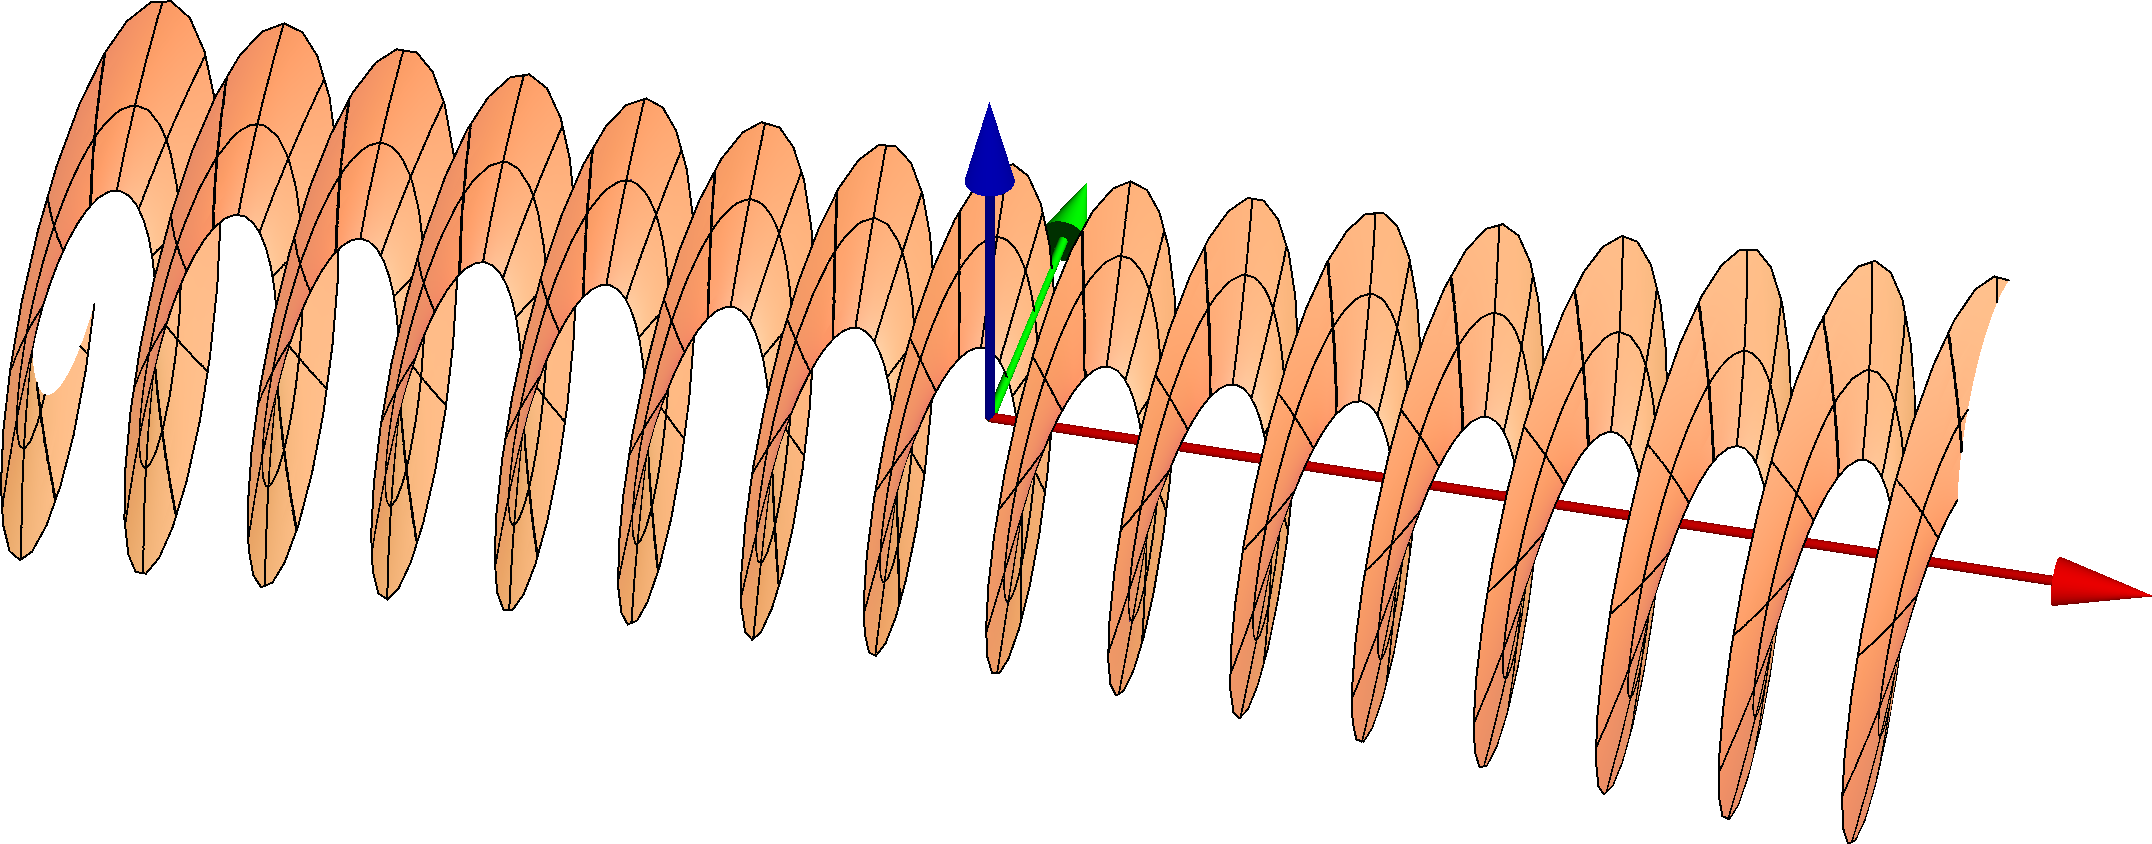
\includegraphics[width=0.7\textwidth]{slike/laguerre_faza}\tabularnewline
\end{tabular}\\
Na sliki je prikazana valovna fronta Gauss-Laguerrovega snopa.}

Poglejmo si še poseben primer omejenega snopa - Besselov snop. Pri
konstrukciji omejenih snopov svetlobe lahko poskusimo sestaviti valovanje,
ki ima ravne fronte. Kot nastavek za rešitev valovne enačbe (\ref{eq:valovna-ena=00010Dba})
lahko izberemo
\begin{equation}
E=E_{0}\psi(x,y)e^{i\beta z},
\end{equation}
kjer mora nastavek $\psi$ zadostovati Helmholtzevi enačbi
\begin{equation}
\nabla_{\perp}^{2}\psi+k_{\perp}^{2}\psi=0,
\end{equation}
kjer je $k_{\perp}^{2}+\beta^{2}=k^{2}$ valovni vektor. V cilindričnih
koordinatah ($x=\rho\cos\phi$, $y=\rho\sin\phi$) se rešitev izraža
z Besselovimi funkcijami:
\begin{equation}
\psi(x,y)=A_{m}J_{m}(k_{\perp}\rho)e^{im\phi},
\end{equation}
kjer je $J_{m}$ Besselova funkcija in $m=0,\pm1,\pm2,\ldots$ Za
$m=0$ ima val kompleksno amplitudo
\begin{equation}
E=A_{0}J_{0}(k_{\perp}\rho)e^{i\beta z},\label{eq:Besselov-snop}
\end{equation}
ki ga imenujemo Besselov snop. Tak snop nima divergence, saj so valovne
fronte ravne, vendar pa ni omejen v pravem smislu. Za velike oddaljenosti
od središča snopa intenzitetni profil pada kot $I=J_{0}^{2}(k_{\perp}\rho)\approx(2/\pi k_{\perp}\rho)\cos^{2}(k_{\perp}\rho-\pi/4)$,
tako da energija takega snopa ni omejena znotraj efektivnega radija,
kot je to pri Gaussovih snopih. Za konstrukcijo Besselovih snopov
bi (tako kot za konstrukcijo ravnega vala) potrebovali neskončno energije.
Približne aproksimacije Besselovih snopov lahko ustvarimo in imajo
pomembne ter uporabne lastnosti v optiki. 

\zanimivo{Ste vedeli?}{Z uporabo stožičaste leče lahko Gaussov snop
transformiramo v približek Besselovega snopa. Poleg manjše divergence
imajo ti snopi še lastnost regeneracije. Snop se bo v senčni strani
za objektom, ki ga osvetljuje, regeneriral. Profil snopa v senčni
strani (daleč stran od objekta) je tako enak tistemu pred objektom.
\medskip{}


\begin{tabular*}{0.01\textwidth}{@{\extracolsep{\fill}}>{\centering}p{0.35\columnwidth}>{\centering}p{0.35\columnwidth}>{\centering}p{0.3\columnwidth}}
\centering\small
\def\svgwidth{0.3\textwidth}
\input{slike/Bessel_beam.pdf_tex}
 & \centering\small
\def\svgwidth{0.3\textwidth}

\input{slike/Bessel_beam_reform.pdf_tex} & \centering\small
\def\svgwidth{0.15\textwidth}

\input{slike/Bessel_beam_intensity.pdf_tex}\tabularnewline
\end{tabular*}}


\section{Transformacije snopov z lečami}

Pri prehodu skozi optične naprave se parametri snopa spremenijo. Začnimo
z enostavno tanko lečo z goriščno razdaljo $f$. V geometrijski optiki
je krivinski radij sferičnega vala, ki izhaja iz točke na osi, kar
enak razdalji do točke. Leča preslika točko na osi v točko na osi,
od tod pa sledi, da se sferični val s krivinskim radijem $R_{1}$
po prehodu skozi lečo spremeni v val s krivinskim radijem $R_{2}$,
pri čemer velja zveza 
\begin{equation}
\frac{1}{R_{1}}-\frac{1}{R_{2}}=\frac{1}{f}.
\end{equation}
Krivinski radij v točki $z$ pozitiven, če je središče pri $z^{\prime}\le z$.

Polmer snopa $w$ se pri prehodu skozi tanko lečo ne spremeni, zato
sledi iz \ref{eq:q-inv}, da velja tudi za kompleksni krivinski radij
tik pred in tik za lečo 
\begin{equation}
\frac{1}{q_{1}}-\frac{1}{q_{2}}=\frac{1}{f}.\label{eq:preslikava-zveza-le=00010Da}
\end{equation}
 Kompleksni krivinski radij je po \ref{eq:q} linearna funkcija $z$.
To nam skupaj z gornjo enačbo \prettyref{eq:preslikava-zveza-le=00010Da}
omogoča račun prehoda snopa skozi poljuben sistem leč brez aberacij.
Kot primer poglejmo, kako z zbiralno lečo ponovno zberemo snop.

\begin{figure}
\centering\small
\def\svgwidth{\textwidth}
\input{slike/preslikava.pdf_tex} \caption{\label{fig:Prehod-Gaussovega-snopa}Prehod Gaussovega snopa skozi
tanko lečo. Grlo velikosti $w_{01}$ v oddaljenosti $x_{1}$ od gorišča
leče se preslika v grlo $w_{02}$ v oddaljenosti $x_{2}$ od gorišča
leče. }
\end{figure}


Vpadni snop naj ima grlo s polmerom $w_{01}$ in dolžino $z_{01}$
v točki, ki je oddaljena za $x_{1}$ od levega gorišča leče (slika
\ref{fig:Prehod-Gaussovega-snopa}). Izračunati želimo položaj in
polmer grla na desni strani leče. Naj bosta 
\begin{equation}
q_{1}^{F}=x_{1}-iz_{01}\mbox{\hskip1cm in \hskip1cm}q_{2}^{F}=-x_{2}-iz_{02}
\end{equation}
 kompleksna krivinska radija v levem in desnem gorišču. Velja tudi
\begin{equation}
q_{1}=q_{1}^{F}+f\mbox{\hskip1cm in \hskip1cm}q_{2}=q_{2}^{F}-f.
\end{equation}
 Od tod dobimo z uporabo \ref{eq:preslikava-zveza-le=00010Da} enačbo
za $q$ v goriščih v kompaktni obliki 
\begin{equation}
q_{1}^{F}q_{2}^{F}=-f^{2},
\end{equation}
 ki je po obliki podobna enačbi za oddaljenost slike od gorišča v
geometrijski optiki, pomen pa ima drugačen. Zapišimo posebej realni
in imaginarni del 
\begin{equation}
x_{1}x_{2}=f^{2}-z_{01}z_{02}
\end{equation}
 in 
\begin{equation}
\frac{x_{1}}{z_{01}}=\frac{x_{2}}{z_{02}}\mbox{\hskip1cm ali \hskip1cm}\frac{w_{01}^{2}}{w_{02}^{2}}=\frac{x_{1}}{x_{2}},\label{eq:preslikava-pove=00010Dava}
\end{equation}
 od koder izračunamo položaj grla na desni: 
\begin{equation}
x_{2}=\frac{x_{1}f^{2}}{x_{1}^{2}+z_{01}^{2}}.\label{eq:preslikava-grlo}
\end{equation}
 Gornja enačba se ujema z izrazom za preslikavo točke v geometrijski
optiki le, kadar je $z_{01}\ll x_{1}$. Kadar je $z_{01}\gg f$, je
val na leči pri vsakem $x_{1}$ skoraj raven in dobimo grlo na desni
v gorišču. V praksi dobimo Gaussove snope iz laserjev in pogosto ne
velja ne prva ne druga limita, temveč je treba uporabiti izraz \ref{eq:preslikava-grlo}.
Tudi povečava polmera grla na desni, podana z \ref{eq:preslikava-pove=00010Dava},
je precej drugačna kot v geometrijski optiki.

Za primer vzemimo snop iz He-Ne laserja, ki ima grlo s polmerom $0.5\usk\milli\metre$
na izhodnem ogledalu in je $50\usk\centi\metre$ pred lečo z $f=25\usk\centi\metre$.
Tedaj je $z_{01}=124\usk\centi\metre$ in po \ref{eq:preslikava-grlo}
dobimo grlo za lečo v oddaljenosti $4\usk\centi\metre$ od gorišča
in s polmerom $0.2\usk\milli\metre$. Enačbe geometrijske optike bi
dale popolnoma napačen položaj grla $25\usk\centi\metre$ za goriščem
s polmerom $0.5\usk\milli\metre$, medtem ko bi približek, da je vpadni
snop kar raven, dal grlo na desni v gorišču s približno pravim polmerom.

Če postavimo grlo snopa v goriščnico leče ($x_{1}=0$) je grlo na
desni strani tudi v goriščnici ($x_{2}=0$). Razmerje polmerov grl
na eni in drugi strani leče je $\lim x_{2}/x_{1}=f^{2}/z_{01}^{2}$.
Velikost grla na desni strani je $w_{02}=\lambda f/(\pi w_{01})$,
torej tem manjša, čim večji je polmer grla na levi, kjer je lahko
največ enak polmeru leče $a$. Najmanjša velikost grla na desni je
tako $\sim\lambda f/a$. Dobri objektivi (mikroskopski in fotografski)
dosegajo numerično odprtino $f/a\simeq1$ in je z njimi Gaussov snop
mogoče zbrati v piko velikosti $\lambda$. Seveda je treba pred lečo
snop dovolj razširiti. To napravimo s teleskopom, ki ga prikazuje
slika \ref{fig:Prehod-Gaussovega-snopa-teleskop}. Povečava teleskopa
je pri taki postavitvi leč kar razmerje med goriščnicama (Naloga \ref{teleskop}).
\begin{figure}
\def\svgwidth{\textwidth}
\input{slike/teleskop.pdf_tex} \caption{\label{fig:Prehod-Gaussovega-snopa-teleskop}Prehod Gaussovega snopa
skozi sistem dveh leč z goriščnicama $f_{1}$ in $f_{2}$, ki sta
na medsebojni razdalji $d=f_{1}+f_{2}$. Tak sistem deluje kot teleskop
s povečavo $\frac{w_{02}}{w_{01}}=\frac{f_{2}}{f_{1}}$.}
\end{figure}


\naloga{teleskop}{Pokaži, da je povečava teleskopa, sestavljenega
iz dveh leč z goriščnicama $f_{1}$ in $f_{2}$, ki sta na medsebojni
razdalji $d=f_{1}+f_{2}$, podana z 
\begin{equation}
\frac{w_{02}}{w_{01}}=\frac{f_{2}}{f_{1}},\label{eq:pove=00010Dava-teleskop}
\end{equation}
neodvisno od postavitve grla snopa $x_{1}$.

}


\section{Linearne racionalne transformacije kompleksnega krivinskega radija}

Gaussove snope povsem opišemo, če v izbrani ravnini $z$ podamo kompleksni
krivinski radij $q$. Ugotovili smo že, da je $q$ linearna funkcija
premika po $z$. Vemo tudi, kako se spremeni pri prehodu skozi tanko
lečo. V tem razdelku skušajmo ta rezultata posplošiti.

Pri premiku iz ravnine $z$ v ravnino $z^{\prime}$, ki je premaknjena
za $d$ , se $q$ spremeni 
\begin{equation}
q^{\prime}=q+d.
\end{equation}
 Po \ref{eq:preslikava-zveza-le=00010Da} je pri prehodu skozi lečo
\begin{equation}
q^{\prime}=\frac{qf}{f-q}=\frac{q}{-\frac{q}{f}+1}.
\end{equation}
 Enako kot leča seveda deluje sferično ogledalo s krivinskim radijem
$R_{0}$, pri katerem je $f=R_{0}/2$. Leča in premik dasta skupaj
\begin{equation}
q^{\prime}=\frac{q}{-\frac{q}{f}+1}+d=\frac{q(1-\frac{d}{f})+d}{-\frac{q}{f}+1}.
\end{equation}


V vseh treh primerih lahko transformacijo $q$ zapišemo v obliki ulomljene
linearne preslikave 
\begin{equation}
q^{\prime}=\frac{Aq+B}{Cq+D}.\label{eq:ulomljena-preslikava}
\end{equation}
 Koeficiente preslikave razvrstimo v matriko 
\begin{equation}
\left[\begin{array}{cc}
A & B\\
C & D
\end{array}\right]
\end{equation}
 Imejmo zaporedje dveh optičnih sistemov s koeficienti $A_{1}$, $B_{1}$,
$C_{1}$, $D_{1}$ in $A_{2}$, $B_{2}$, $C_{2}$, $D_{2}$. Brez
težav se prepričamo, da je skupna transformacija zopet oblike \ref{eq:ulomljena-preslikava}
in da jo dobimo z množenjem matrik posameznih sistemov: 
\begin{eqnarray}
\left[\begin{array}{cc}
A & B\\
C & D
\end{array}\right] & = & \left[\begin{array}{cc}
A_{2} & B_{2}\\
C_{2} & D_{2}
\end{array}\right]\cdot\left[\begin{array}{cc}
A_{1} & B_{1}\\
C_{1} & D_{1}
\end{array}\right]\nonumber \\
 & = & \left[\begin{array}{cc}
A_{2}A_{1}+B_{2}C_{1} & A_{2}B_{1}+B_{2}D_{1}\\
C_{2}A_{1}+D_{2}C_{1} & C_{2}B_{1}+D_{2}D_{1}
\end{array}\right].
\end{eqnarray}


Gornji matrični formalizem je zelo prikladen za računanje zapletenih
optičnih sistemov, saj ga je prav lahko izvesti na računalnik. Poleg
tega je enolično povezan z matričnim formalizmom v geometrijski optiki
in daje možnost prenosa rezultatov računov geometrijske optike v optiko
snopov.
\begin{figure}
\centering\small\input{slike/k_preslikavam.pdf_tex}

\centering\small\input{slike/k_matrikam.pdf_tex}

\caption{\label{fig:K-matri=00010Dni-obravnavi}Preslikave žarkov lahko obravnavamo
z matrikami. Optični element $M$ preslika žarek $(y_{1},\theta_{1})$
v $(y_{2},\theta_{2})$. Matriko za prehod poljubnega zaporedja optičnih
elementov dobimo z množenjem matrik.}
\end{figure}


Sliko v geometrijski optiki dobimo kot presečišče geometrijskih žarkov,
ki izhajajo iz točke predmeta pred optičnim sistemom. Geometrijski
žarek je normala na valovne ploskve, pri čemer moramo vzeti še limito,
ko gre valovna dolžina proti nič. Ukrivljenost valovne fronte je neposredno
povezana s spreminjanjem naklona žarkov. Snop žarkov geomtrijske optike,
ki izhajajo iz točke, ustreza snopu valovanja, pri katerem pa je premer
grla končen. Če naj se v točki slike zberejo vsi žarki, če naj so
torej napake leč majhne, seveda nakloni žarkov glede na os ne smejo
biti veliki.

Žarek lahko v izbrani ravnini $z$ opišemo z oddaljenostjo od osi
$y$ in s strmino glede na os $\theta$. Iz teh dveh količin tvorimo
stolpec 
\begin{equation}
\left[\begin{array}{c}
y\\
\theta
\end{array}\right].
\end{equation}


Iz slike \ref{fig:K-matri=00010Dni-obravnavi} razberemo, da se pri
premiku za $d$ spremeni le odmik od osi 
\begin{equation}
\left[\begin{array}{c}
y_{2}\\
\theta_{2}
\end{array}\right]=\left[\begin{array}{c}
y_{1}+d\theta_{1}\\
\theta_{1}
\end{array}\right],
\end{equation}
 kar lahko zapišemo v matrični obliki 
\begin{equation}
\left[\begin{array}{c}
y_{2}\\
\theta_{2}
\end{array}\right]=\left[\begin{array}{cc}
1 & d\\
0 & 1
\end{array}\right]\cdot\left[\begin{array}{c}
y_{1}\\
\theta_{1}
\end{array}\right].
\end{equation}
 Pri prehodu skozi tanko lečo se spremeni nagib žarka. Če je pred
lečo vzporeden z osjo, gre za lečo skozi gorišče, zato 
\begin{equation}
\left[\begin{array}{c}
y_{2}\\
\theta_{2}
\end{array}\right]=\left[\begin{array}{c}
y_{1}\\
-\frac{y_{1}}{f}
\end{array}\right]=\left[\begin{array}{cc}
1 & B\\
-\frac{1}{f} & D
\end{array}\right]\cdot\left[\begin{array}{c}
y_{1}\\
0
\end{array}\right].
\end{equation}
 Žarek, ki gre na osi skozi lečo, ostane nespremenjen; to nam da koeficienta
$B$ in $D$: 
\begin{equation}
\left[\begin{array}{c}
y_{2}\\
\theta_{2}
\end{array}\right]=\left[\begin{array}{c}
0\\
\theta_{1}
\end{array}\right]=\left[\begin{array}{cc}
1 & B\\
-\frac{1}{f} & D
\end{array}\right]\cdot\left[\begin{array}{c}
0\\
\theta_{1}
\end{array}\right].
\end{equation}
 Sledi $B=0$ in $D=1$. Matrika za prehod skozi lečo je tako 
\begin{equation}
\left[\begin{array}{cc}
1 & 0\\
-\frac{1}{f} & 1
\end{array}\right]
\end{equation}
in je enaka kot matrika transformacije kompleksnega krivinskega radija
za tanko lečo. Matriko sestavljene optične naprave očitno dobimo z
množenjem matrik komponent. Tako je tudi splošno matrika za transformacijo
parametrov žarka v geometrijski optiki enaka kot transformacija kompleksne
ukrivljenosti v optiki snopov. Matrike za nekaj osnovnih preslikav
so podane na sliki \ref{fig:Matrike-za-preslikave}. 
\begin{figure}
\subfloat[Prehod skozi prostor.]{%
\begin{tabular}{>{\centering}m{0.2\textwidth}c}
\centering\small\input{slike/matrika_d.pdf_tex} & $M=\left[\begin{array}{cc}
1 & d\\
0 & 1
\end{array}\right]$\tabularnewline
\end{tabular}

}\hfill{}\subfloat[Prehod preko meje $n_{1}$, $n_{2}$. \hfill{}]{%
\begin{tabular}{>{\centering}m{0.2\textwidth}c}
\centering\small\input{slike/matrika_n.pdf_tex} & $M=\left[\begin{array}{cc}
1 & 0\\
0 & \frac{n_{1}}{n_{2}}
\end{array}\right]$\tabularnewline
\end{tabular}

}

\subfloat[Prehod preko konveksno ukrivljene meje: $R>0$.]{%
\begin{tabular}{>{\centering}m{0.2\textwidth}c}
\centering\small\input{slike/matrika_nR.pdf_tex} & $M=\left[\begin{array}{cc}
1 & 0\\
\frac{(n_{1}-n_{2})}{n_{2}R} & \frac{n_{1}}{n_{2}}
\end{array}\right]$\tabularnewline
\end{tabular}

}\hfill{}\subfloat[Prehod preko konveksne leče: $f>0$.]{%
\begin{tabular}{>{\centering}m{0.2\textwidth}c}
\centering\small\input{slike/matrika_f.pdf_tex} & $M=\left[\begin{array}{cc}
1 & 0\\
-\frac{1}{f} & 1
\end{array}\right]$\tabularnewline
\end{tabular}

}

\subfloat[Odboj na ravnem zrcalu: spremeni smer.]{%
\begin{tabular}{>{\centering}m{0.2\textwidth}c}
\centering\small\input{slike/matrika_I.pdf_tex} & $M=\left[\begin{array}{cc}
1 & 0\\
0 & 1
\end{array}\right]$\tabularnewline
\end{tabular}

}\hfill{}\subfloat[Odboj od konkavnega zrcala: $R>0$.]{%
\begin{tabular}{>{\centering}m{0.2\textwidth}c}
\centering\small\input{slike/matrika_R.pdf_tex} & $M=\left[\begin{array}{cc}
1 & 0\\
-\frac{2}{R} & 1
\end{array}\right]$\tabularnewline
\end{tabular}

}

\caption{\label{fig:Matrike-za-preslikave}Matrike za osnovne preslikave v
geometrijski optiki lahko uporabimo za izračun preslikave kompleksnega
krivinskega radija $q$ Gaussovih snopov. Odboj od zrcala s krivinskim
radijem $R$ je ekvivalenten preslikavi leče z goriščnico $f=R/2$.}
\end{figure}


\naloga{naloga-leča}{Pokaži, da so matrike za prehod prostor-leča,
za lečo z lomnim količnikom $n$, debeline $d$ in krivinskima radijema
$R_{1}$ in $R_{2}$, ter za prehod čez zaporedje sredstev z različnimi
lomnimi količniki podane z\medskip{}


\begin{tabular*}{1\textwidth}{@{\extracolsep{\fill}}>{\centering}m{0.2\textwidth}>{\centering}p{0.6\linewidth}>{\centering}p{0.2\linewidth}}
\small\input{slike/matrika_df.pdf_tex} & $M=\left[\begin{array}{cc}
1 & d\\
-\frac{1}{f} & 1-\frac{d}{f}
\end{array}\right]$, & \tagarray\label{space-lens}\tabularnewline
\small\input{slike/matrika_fd.pdf_tex} & $M=\left[\begin{array}{cc}
1-\frac{d}{nf_{1}} & \frac{d}{n}\\
-\frac{f_{1}+f_{2}}{f_{1}f_{2}}+\frac{d}{nf_{1}f_{2}} & 1-\frac{d}{nf_{2}}
\end{array}\right];\; f_{i}=\frac{R_{i}}{n-1},$ & \tagarray\label{thick-lens}\tabularnewline
\scriptsize\input{slike/matrika_nN.pdf_tex} & $M=\left[\begin{array}{cc}
1 & \sum_{i=1}^{N}\frac{d_{i}}{n_{i}}\\
0 & 1
\end{array}\right]$. & \tagarray\tabularnewline
\end{tabular*}

}
\end{document}
